\documentclass{article}
\usepackage[MeX]{polski}
\usepackage[utf8]{inputenc}
\usepackage{amsfonts}
\usepackage{amssymb}
\usepackage{graphicx}
\usepackage[pdftex]{color,graphicx}

\author{Piotr Dobrowolski}
\title{Raport \\{\small Projekt Zaliczeniowy z Rachunku Prawdopodobieństwa i Statystyki} }
\date{\today}
\frenchspacing

\begin{document}
\maketitle
\tableofcontents
\section{O testowaniu}
\subsection{Założenia}
Testowanie strategii w moim projekcie odbywa się poprzez wielokrotne symulowanie kupowania
obiadów przez klientów. Podejście do testowania: 1-wizualizajca danej, konkretnej, symulacji, oraz 2-
wielokrotne symulowanie - szukanie najgorszych danych wejściowych.
\subsection{Symulacja}
\paragraph{symulacja = function(M, k, Grupy, strategia, wypisuj = 0)::} Dla danych parametrów M, k, Grupy, strategia
funkcja przeprowadza symulacje kupowania obiadów przez klientów. Każdy klient (wszystkich jest N) przychodzi codziennie
do bufetu i kupuje, bądź też nie, obiad. Każdego dnia pyta się strategii o koszt, a pod koniec dnia przekazuje
strategii ilość kupionych obiadów.
\subsection{Konkretna symulacja - testowanie}
Testowanie strategii na jednej, konkretnej symulacji. Polega na porównaniu działania strategii do strategii optymalnej
i losowej, gdzie optymalna (opisana później) stanowi pewne maksimum do którego chcę, aby dążyła (w przeciągu dni) testowana strategia
, a losowa minimum. 
\paragraph{test\_LO = function(M, k, Grupy, strategia, metoda\_symulacji)::} Funkcja tworzy wykresy porównujące wybraną
strategię do optymalnej i losowej. Dzięki temu można przeanalizować jak w czasie (dni) działa dana strategia. Wypisywane jest także
podsumowanie zysków każdego dnia, oraz zysk całkowity, uzyskany przez M dni.
\subsection{Grupy testów}
\paragraph{testy\_szukaj\_najgorszych\_M = function(Grupy, k, strategia, metoda\_symulacji, wypisuj = 0)::} Funkcja testuje strategię
ze względu na radzenie sobie z różną ilością dni. Chodzi o to żeby strategia jak najszybciej umożliwiała dobrać
najlepszy koszt.
\paragraph{testy\_szukaj\_najgorszych = function(strategia, metoda\_symulacji, wypisuj = 0)::} Funkcja wykorzystuje tę powyższą, ale teraz
wykonuje testy dla różnych grup klientów, które dobiera losowo. Dzięki niej można określić (i zmieniając parametry funkcji powyższej
, czyli ilości dni jakie będą testowane) dla jakich ilości dostępnych dni, oraz dla jakich grup strategia najgorzej sobie radzi.
\\ Dzięki tej funkcji (przy parametrze wypisuj > 0) można także uzyskać informacje o atomowych testach występujących w tej grupie testów
. Dzięki temu można przeanalizować daną strategię.

\section{Strategie - opis, testy i problemy}
Poniżej znajduje się jakie użyłem do zmaksymalizowania zysku.
Nietrywialne strategie starają się estymować nie wartości wszystkich parametrów dla każdej grupy klientów, tylko 
jeden parametr - koszt oczekiwany.

\subsection{Strategie do testowania}
\paragraph{Strategia - losuję koszt każdego dnia}
Strategia losująca koszt służy do porównania. Koszt wybierany jest z rozkładem jednostajnym.
\paragraph{Strategie - optymalna, znam grupy}
Jeżeli grupy klientów są znane, to najbardziej opłacalną strategią jest wybranie jednego kosztu z \{0, $\alpha_1$, $\alpha_2$,
   $\alpha_3$, $\alpha_4$, $\alpha_5$\} (odpowiednio mniej jeżeli mniej grup). Dla każdego z tych kosztów liczę wartość oczekiwaną
   zysku. Wybieram ten koszt, dla którego ta jest największa.
\subsection{Strategia 'szukam'}
Strategia dzieli liczbę dni (M) na \textit{podzial\_na} równych części. Następnie (dla kolejnej części -dni) 
przeszukuje równomiernie przedział kosztów (początkowo cały od $0$ do $C$) i zapisuje maksimum zysku i koszt, gdzie wystąpiło.
Następnie, po przejściu tej części dni, następuje zmiana przedziału na taki gdzie odległość od maksimum, które wystąpiło
wynosi dwie długości przedziału (kosztu). Zawsze zawężam bardzo mocno przedział.
\subsection{Analiza strategii 'szukam'}
Strategia źle sobie radzi dla bardzo małych M, dlatego w przypadku wystąpienia M < 10 zostaje wywołana strategia losowa.
\paragraph{Pięta achillesowa strategii}
Koszt podawany przez strategię estymuje w okolicach dobrego, mniej więcej równo dowartościowuje i
niedowartościowuje, jednak zysk w przypadku za dużego kosztu / za małego może się diametralnie zmieniać. Przez co,
jeżeli maksimum jakie wystąpiło będzie znacząco odbiegało od rzeczywistego to niedokładności będą większe. 
A jeżeli koszt zostanie obliczony poniżej oczekiwanego może zdarzyć się, że już nie wróci do poprawnego, przez co zysk będzie bardzo
kiepski. Taką sytuację przedstawiają wykresy poniżej:
\begin{center}
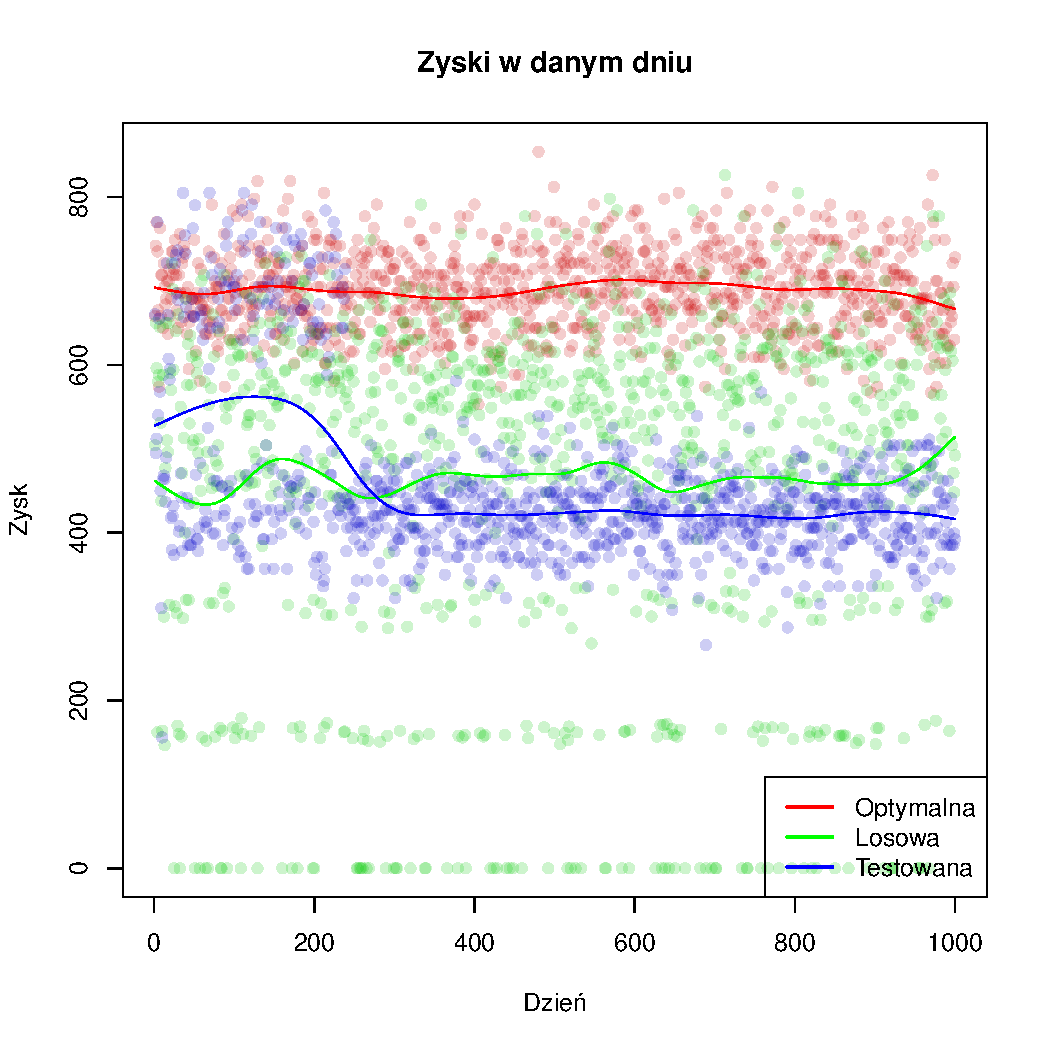
\includegraphics[scale=0.52]{wykresy/problemy/Zysk_strategii_porownanie_koszt_troche_za_maly.pdf}
\end{center}
\begin{center}
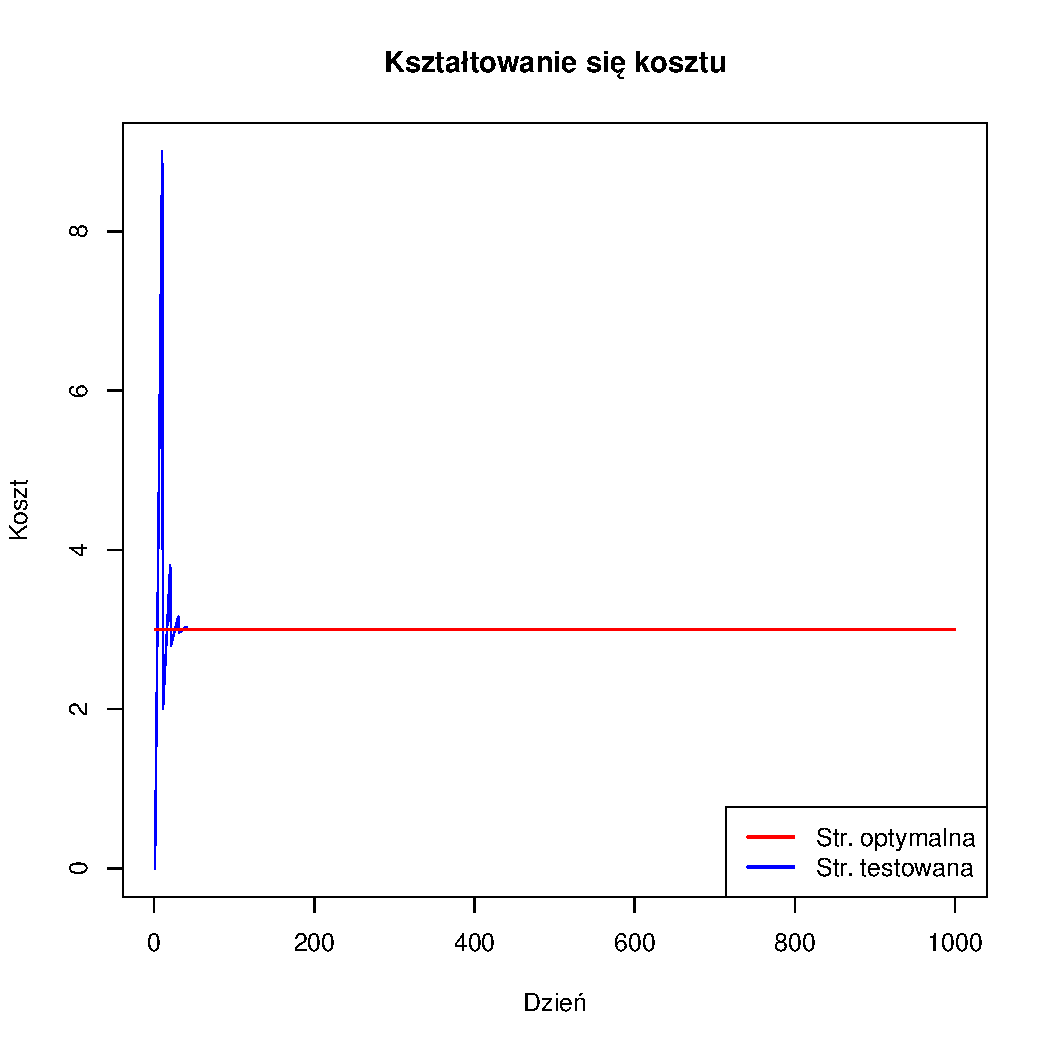
\includegraphics[scale=0.52]{wykresy/problemy/Ksztaltowanie_sie_kosztu_troche_za_maly.pdf}
\end{center}
\paragraph{Dobranie parametru \textit{podzial\_na}}
Na tym przykładzie pokażę jak dobierałem parametry, tak samo dla innych strategii. Dla każdej
nie chcę umieszczać w raporcie z powodu strasznego wsrostu objętości tego raportu.

Przykład dla grup poniżej, M=1000 i M=100:\\
c.0..0..0. c.0..0..0..1 c.0..0..0..2 c.0..0..0..3 c.0..0..0..4\\
1 0.68496002    6.1336505    5.3973523    8.3772073    9.4554115\\
2 0.07742254    0.4397591    0.4052306    0.3738446    0.4736273\\
3 0.94539217    0.6658948    0.6140436    0.8749763    0.7579729\\

Wyniki dla parametru = 
\paragraph{\textit{podzial\_na}=3} 
\begin{center}
\includegraphics[scale=0.5]{wykresy/szukamz1.pdf}
\includegraphics[scale=0.5]{wykresy/szukamk1.pdf}
\\
\includegraphics[scale=0.5]{wykresy/szukamz2.pdf}
\includegraphics[scale=0.5]{wykresy/szukamk2.pdf}
\end{center}
Wynik dla M=1000:\\
 "ZYSKI:"\\
 "Strategia optymalna"\\
   Min. 1st Qu.  Median    Mean 3rd Qu.    Max. \\
  959.4  1127.0  1174.0  1177.0  1230.0  1397.0 \\
 "Całkowity:  1176908.72583089 zł"\\
 "Strategia losowa"\\
    Min.  1st Qu.   Median     Mean  3rd Qu.     Max. \\
   1.945  365.500  631.600  624.800  876.500 1308.000 \\
 "Całkowity:  624790.202300427 zł"\\
 "Strategia testowana"\\
   Min. 1st Qu.  Median    Mean 3rd Qu.    Max. \\
    490    1070    1114    1108    1153    1334 \\
 "Całkowity:  1107608.11288623 zł"\\
\\
Wynik dla M=100\\
 "ZYSKI:"\\
 "Strategia optymalna"\\
   Min. 1st Qu.  Median    Mean 3rd Qu.    Max. \\
   1034    1136    1174    1173    1204    1351\\ 
 "Całkowity:  117304.298424064 zł"\\
 "Strategia losowa"\\
    Min.  1st Qu.   Median     Mean  3rd Qu.     Max. \\
   2.915  332.000  674.400  634.900  905.700 1184.000\\ 
 "Całkowity:  63486.6311215423 zł"\\
 "Strategia testowana"\\
   Min. 1st Qu.  Median    Mean 3rd Qu.    Max. \\
  463.3  1050.0  1118.0  1083.0  1157.0  1231.0\\ 
 "Całkowity:  108312.561033286 zł"\\
 
 
 \paragraph{\textit{podzial\_na}=5} 
 \begin{center}
 \includegraphics[scale=0.5]{wykresy/szukamz3.pdf}
 \includegraphics[scale=0.5]{wykresy/szukamk3.pdf}
 \\
 \includegraphics[scale=0.5]{wykresy/szukamz4.pdf}
 \includegraphics[scale=0.5]{wykresy/szukamk4.pdf}
 \end{center}
 
Wynik dla M=1000:\\
"ZYSKI:"\\
"Strategia optymalna"\\
Min. 1st Qu.  Median    Mean 3rd Qu.    Max.  \\
987.4  1136.0  1183.0  1179.0  1220.0  1388.0  \\
"Całkowity:  1179060.50006546 zł" \\
"Strategia losowa" \\
Min.  1st Qu.   Median     Mean  3rd Qu.     Max.  \\
1.226  344.500  619.200  619.700  873.700 1311.000  \\
"Całkowity:  619651.431804753 zł" \\
"Strategia testowana" \\
Min. 1st Qu.  Median    Mean 3rd Qu.    Max.  \\
302    1095    1140    1135    1185    1364 \\ 
"Całkowity:  1135266.45900154 zł" \\

Wynik dla M=100:\\
"ZYSKI:" \\
"Strategia optymalna" \\
Min. 1st Qu.  Median    Mean 3rd Qu.    Max.  \\ 
1025    1143    1192    1188    1232    1304  \\
"Całkowity:  118841.280020187 zł" \\
"Strategia losowa" \\
Min. 1st Qu.  Median    Mean 3rd Qu.    Max.  \\
12.62  320.00  571.40  588.40  864.20 1289.00 \\ 
"Całkowity:  58840.8354558563 zł" \\
"Strategia testowana" \\
Min. 1st Qu.  Median    Mean 3rd Qu.    Max.  \\
300    1113    1166    1125    1218    1311 \\ 
"Całkowity:  112546.93516384 zł" \\

\paragraph{\textit{podzial\_na}=15}
\begin{center}
\includegraphics[scale=0.5]{wykresy/szukamz5.pdf}
\includegraphics[scale=0.5]{wykresy/szukamk5.pdf}
\\
\includegraphics[scale=0.5]{wykresy/szukamz6.pdf}
\includegraphics[scale=0.5]{wykresy/szukamk6.pdf}
\end{center}

Wynik dla M=1000:\\

"ZYSKI:" \\
"Strategia optymalna" \\
Min. 1st Qu.  Median    Mean 3rd Qu.    Max.  \\
996.7  1136.0  1183.0  1181.0  1220.0  1369.0 \\ 
"Całkowity:  1181435.83525947 zł" \\
"Strategia losowa" \\
Min.  1st Qu.   Median     Mean  3rd Qu.     Max.  \\
4.625  365.600  608.900  606.800  851.400 1310.000  \\
"Całkowity:  606752.627675668 zł" \\
"Strategia testowana" \\
Min. 1st Qu.  Median    Mean 3rd Qu.    Max.  \\
0    1103    1158    1145    1195    1377 \\ 
"Całkowity:  1144982.43068307 zł" \\

Wynik dla M=100:\\
"ZYSKI:" \\
"Strategia optymalna" \\
Min. 1st Qu.  Median    Mean 3rd Qu.    Max.  \\
1025    1127    1174    1173    1220    1360 \\ 
"Całkowity:  117267.038264158 zł" \\
"Strategia losowa" \\
Min. 1st Qu.  Median    Mean 3rd Qu.    Max.  \\
10.99  442.90  659.10  644.30  879.20 1198.00 \\ 
"Całkowity:  64427.8552497155 zł" \\
"Strategia testowana" \\
Min. 1st Qu.  Median    Mean 3rd Qu.    Max.  \\
0    1035    1115    1042    1170    1325 \\ 
"Całkowity:  104198.498181267 zł" \\

\paragraph{\textit{podzial\_na}=M/10}
\begin{center}
\includegraphics[scale=0.5]{wykresy/szukamz7.pdf}
\includegraphics[scale=0.5]{wykresy/szukamk7.pdf}
\\
\includegraphics[scale=0.5]{wykresy/szukamz8.pdf}
\includegraphics[scale=0.5]{wykresy/szukamk8.pdf}
\end{center}

Wynik dla M=1000:\\
"ZYSKI:" \\
"Strategia optymalna" \\
Min. 1st Qu.  Median    Mean 3rd Qu.    Max.  \\
987.4  1136.0  1174.0  1177.0  1220.0  1379.0 \\ 
"Całkowity:  1177206.80711014 zł" \\
"Strategia losowa" \\
Min.  1st Qu.   Median     Mean  3rd Qu.     Max.  \\
3.212  342.200  632.900  624.500  897.100 1291.000  \\
"Całkowity:  624518.963521281 zł" \\
"Strategia testowana" \\
Min. 1st Qu.  Median    Mean 3rd Qu.    Max.  \\
0    1051    1104    1059    1148    1279 \\ 
"Całkowity:  1059039.08604572 zł" \\


Wynik dla M=100:\\
"ZYSKI:" \\
"Strategia optymalna" \\
Min. 1st Qu.  Median    Mean 3rd Qu.    Max.  \\
1006    1136    1178    1178    1220    1369 \\ 
"Całkowity:  117760.735382913 zł" \\
"Strategia losowa" \\
Min.  1st Qu.   Median     Mean  3rd Qu.     Max.  \\
4.622  339.800  602.300  602.300  870.300 1207.000  \\
"Całkowity:  60227.792022333 zł" \\
"Strategia testowana" \\
Min. 1st Qu.  Median    Mean 3rd Qu.    Max.  \\
165    1057    1128    1083    1183    1302 \\ 
"Całkowity:  108298.784623616 zł" \\

\subsection{Strategia 'szukam' wnioski}   
Jak widać dla parametru zależnego od M wynik niekoniecznie jest dobry ponieważ bardzo dużo czasu traci się na 
zbieranie informacji, które i tak nie muszą prowadzić do lepszego wyniku - np przedstawia to wykres dla M=1000.
Z testów wynika, że najlepiej się sprawdzał parametr równy około 15. Jednak dla przypadków granicznych - gdy jest wyłącznie
grupa gdzie $\alpha = 9.9, p^+ = 1, p^- = 0$, które w sytuacji rzeczywistej ciężko by było znaleźć, jedynie gdy podział jest bardzo
gęsty można wychwycić tą sytuację. Nie zostanie ona wychwycona, ponieważ zysk w przypadku kosztów = 10 zawsze jest 0, a
strategia stara się zmaksymalizować koszty, nie patrzy na ilość kupionych obiadów bezpośrednio.

Analiza testów zbiorowych pokazuje to, że strategia wybiera dość często złą wartość, która jest bardzo blisko tej właściwej.


R: \textit{testy\_szukaj\_najgorszych(strategia\_szukam, symulacja)}
\subsection{Strategia 'szukam\_wyzej' wnioski}

Jest to strategia, która ma za zadanie jak najbardziej przybliżać koszt oczekiwany, jednocześnie nie 
spadając poniżej wartości granicznej, ponieważ $p^+ > p^-$ lepiej jest być powyżej wartości.
. Jest analogiczna to powyższej, jednak dzięki tej małej zmianie znacznie lepiej sobie radzi.
Teraz nowy podział jest w stosunku 3:2 nad kosztem maksymalnym:pod kosztem maksymalnym.

\subsection{Strategia ide\_gdzie\_lepiej\_2}
Strategia składa się z 2 faz:
\paragraph{1:} pobieranie informacji przez x dni.\\
w tej fazie przez x dni, gdzie x jest parametrem strategii będę szukał kosztu dającego największy zysk.
Będzie to mało inteligentne przeszukiwanie kosztów, od najmniejszego do największego.
\paragraph{2:} ulepszanie\\
Teraz będę przemieszczał się o $\Delta$ codziennie z kosztem, w kierunku wzrastającego zysku.

Przykład R: \textit{test\_LO(1000, 5, generuj\_grupy(5), strategia\_ide\_gdzie\_lepiej\_2, symulacja)}\\
Testy dla wielu parametrów R: \textit{testy\_szukaj\_najgorszych(strategia\_ide\_gdzie\_lepiej\_2, symulacja, 2)}\\

\subsection{Strategia ide\_gdzie\_lepiej\_2 przykładowe wyniki}
Wyniki dla małych M, z którymi strategia sobie dość dobrze radzi, (dla $\Delta = 0.3$, poczatek = 5, M=20) :
\begin{center}
\includegraphics[scale=0.5]{wykresy/lepiejz1.pdf}
\includegraphics[scale=0.5]{wykresy/lepiejk1.pdf}
\end{center}

   Min. 1st Qu.  Median    Mean 3rd Qu.    Max. \\
  822.1   893.3   944.1   934.8   970.6  1009.0 \\
"Całkowity:  18695.5393770244 zł"\\
"Strategia losowa"\\
   Min. 1st Qu.  Median    Mean 3rd Qu.    Max. \\
  44.34  408.80  717.20  610.30  782.70  907.00 \\
"Całkowity:  12206.1772781494 zł"\\
"Strategia testowana"\\
   Min. 1st Qu.  Median    Mean 3rd Qu.    Max. \\
  0.211 734.000 817.600 741.200 893.200 931.700 \\
"Całkowity:  14824.811 zł"\\

\subsection{Strategia ide\_gdzie\_lepiej\_2 przykładowe problemy}
Strategia przekracza granicę bardzo często (średnio co 4 jeżeli jest w pobliżu niej) co nie jest dobre. Jak na wykresie:
\begin{center}
\includegraphics[scale=0.5]{wykresy/lepiejz2.pdf}
\includegraphics[scale=0.5]{wykresy/lepiejk2.pdf}
\end{center}

Można temu zaradzić 
podobnie jak różniły się strategie 'szukam' od 'szukam\_wyzej' priorytet dając poszukiwaniom wyższych kosztów.
Tą strategię można także poprawić w ten sposób, że zamiast 1 maksimum wybieramy parę (ale niedużo 3-4) różne punktu z zakresu
kosztów od 0zł do C=10zł i zrobić osobne przeszukiwania.

\section{Wnioski}
Strategia 'szukam' w średnim przypadku nie daje złych wyników. Jednak narażona jest na klęskę w niektórych przypadkach. 
Następna strategia 'szukam\_wyzej' jest lepiej uodporniona na przypadki gwałtownego spadku zysków poniżej granicy kosztów.
Strategia ide\_gdzie\_lepiej\_2 jest przygotowana na sprajne przypadki. Ma możliwości kalibracji przez większą ilość parametrów, 
przez co staje się bardziej skalowalna (przygotowana na większą ilość\/ mniejszą ilość dni). 

\end{document}
